% !TeX program = xelatex
\documentclass[aspectratio=169,11pt]{beamer}
\usepackage{lmodern,fontspec}
\IfFontExistsTF{Arial}{\setsansfont{Arial}}{\setsansfont{TeX Gyre Heros}}
\usefonttheme{professionalfonts}
\usepackage[absolute,overlay]{textpos}
\usepackage{amsmath,amssymb,array,booktabs,colortbl,graphicx}
\definecolor{navy}{HTML}{142D45}
\definecolor{paper}{HTML}{FAFCFE}
\definecolor{paleblue}{HTML}{DDEBFA}
\definecolor{paleteal}{HTML}{D9EFEA}
\setbeamercolor{background canvas}{bg=paper}
\setbeamercolor{normal text}{fg=navy}
\setbeamercolor{itemize item}{fg=navy}
\setbeamertemplate{navigation symbols}{}
\setbeamertemplate{footline}{}
\setbeamertemplate{itemize item}{\raisebox{0.1ex}{\scriptsize\textbullet}}
\setbeameroption{hide notes}
\setbeamertemplate{note page}[plain]
\graphicspath{{assets/}}
\setlength{\TPHorizModule}{1mm}
\setlength{\TPVertModule}{1mm}
\begin{document}

% Slide 1: AdvNet
% AdvNet paper §1–3
\begin{frame}[plain]
\begin{textblock*}{144mm}(8mm,12mm)
\raggedright\color[HTML]{142D45}\fontsize{34}{41.82}\selectfont \bfseries AdvNet
\end{textblock*}
\begin{textblock*}{144mm}(8mm,35mm)
\raggedright\color[HTML]{142D45}\fontsize{17}{20.91}\selectfont Revealing Performance Issues in Network Protocols\par by Generating Adversarial Environments
\end{textblock*}
\begin{textblock*}{144mm}(8mm,65mm)
\raggedright\color[HTML]{2869B3}\fontsize{12}{14.76}\selectfont Motivation, search design, and practical use cases
\end{textblock*}
\begin{textblock*}{144mm}(8mm,81mm)
\raggedright\color[HTML]{526474}\fontsize{6.3}{7.749}\selectfont Shehab Sarar Ahmed et al. Proc. ACM Netw. 4, CoNEXT2, Article 12 (2026).
\end{textblock*}
\end{frame}
\note{Today, we will introduce AdvNet, a system for adversarially testing network protocols, especially Congestion Control. The question is simple: even if a protocol works well in existing tests, can we automatically find network conditions where it performs much worse?\par \par I'll start with the motivation and how AdvNet works, focusing on its search design.
\par\smallskip Source: AdvNet paper §1–3}


% Slide 2: Bandwidth and throughput
% AdvNet paper §1–3
\begin{frame}[plain]
\begin{textblock*}{144mm}(8mm,6mm)
\raggedright\color[HTML]{142D45}\fontsize{22}{27.06}\selectfont \bfseries Bandwidth and throughput
\end{textblock*}
\begin{textblock*}{30mm}(9mm,26mm)
\raggedright\color[HTML]{2869B3}\fontsize{17}{20.91}\selectfont \bfseries Sender
\end{textblock*}
\begin{textblock*}{53mm}(56mm,26mm)
\raggedright\color[HTML]{087F82}\fontsize{16}{19.68}\selectfont \bfseries Bottleneck queue
\end{textblock*}
\begin{textblock*}{32mm}(120mm,26mm)
\raggedright\color[HTML]{2869B3}\fontsize{17}{20.91}\selectfont \bfseries Receiver
\end{textblock*}
\begin{textblock*}{12mm}(41mm,26mm)
\raggedright\color[HTML]{142D45}\fontsize{18}{22.14}\selectfont →
\end{textblock*}
\begin{textblock*}{10mm}(108mm,26mm)
\raggedright\color[HTML]{142D45}\fontsize{18}{22.14}\selectfont →
\end{textblock*}
\begin{textblock*}{117mm}(34mm,42mm)
\raggedright\color[HTML]{526474}\fontsize{11}{13.53}\selectfont ACK feedback returns to the sender
\end{textblock*}
\begin{textblock*}{144mm}(8mm,56mm)
\raggedright\color[HTML]{142D45}\fontsize{10.5}{12.915}\selectfont \begin{itemize}\setlength{\itemsep}{2.6mm}\setlength{\parskip}{0pt}
\item Bandwidth is link capacity; throughput is the achieved rate
\item Sending too slowly leaves capacity unused
\item Sending too quickly builds queues and increases delay
\end{itemize}
\end{textblock*}
\begin{textblock*}{144mm}(8mm,83mm)
\raggedright\color[HTML]{526474}\fontsize{7}{8.61}\selectfont RTT: round-trip time.
\end{textblock*}
\end{frame}
\note{First, a little background. Bandwidth describes the capacity of a link. Throughput describes the rate that the protocol actually achieves. For a continuously backlogged flow with no other bottleneck, the goal is to make throughput close to the available capacity.\par \par The problem is a sender usually does not know how much bandwidth it can use. Sending too slowly wastes capacity. Sending too quickly builds a queue and increases delay.
\par\smallskip Source: AdvNet paper §1–3}


% Slide 3: What controls TCP sending?
% AdvNet paper §1–3
\begin{frame}[plain]
\begin{textblock*}{144mm}(8mm,6mm)
\raggedright\color[HTML]{142D45}\fontsize{22}{27.06}\selectfont \bfseries What controls TCP sending?
\end{textblock*}
\begin{textblock*}{68mm}(8mm,25mm)
\raggedright\color[HTML]{2869B3}\fontsize{12}{14.76}\selectfont \bfseries Sending controls
\end{textblock*}
\begin{textblock*}{69mm}(8mm,37mm)
\raggedright\color[HTML]{142D45}\fontsize{12}{14.76}\selectfont \begin{itemize}\setlength{\itemsep}{2.6mm}\setlength{\parskip}{0pt}
\item Congestion window limits unacknowledged data in flight
\item Pacing controls packet departure timing
\end{itemize}
\end{textblock*}
\begin{textblock*}{68mm}(85mm,25mm)
\raggedright\color[HTML]{087F82}\fontsize{12}{14.76}\selectfont \bfseries Feedback and recovery
\end{textblock*}
\begin{textblock*}{67mm}(85mm,37mm)
\raggedright\color[HTML]{142D45}\fontsize{11.5}{14.145}\selectfont \begin{itemize}\setlength{\itemsep}{2.6mm}\setlength{\parskip}{0pt}
\item ACK processing
\item Duplicate ACKs and fast retransmit
\item Retransmission timeout (RTO)
\end{itemize}
\end{textblock*}
\end{frame}
\note{Two mechanisms help control sending. The congestion window limits how much unacknowledged data can be in flight. Pacing controls how quickly packets leave the sender. A fast path with a long round-trip time usually needs more data in flight, thus bigger cwnd, to stay busy. In addition, acknowledgment and retransmission logic—such as duplicate ACKs and retransmission timeouts (RTO)—also directly affect performance.
\par\smallskip Source: AdvNet paper §1–3}


% Slide 4: Why congestion control is hard to test
% AdvNet paper §1–3
\begin{frame}[plain]
\begin{textblock*}{144mm}(8mm,6mm)
\raggedright\color[HTML]{142D45}\fontsize{22}{27.06}\selectfont \bfseries Why congestion control is hard to test
\end{textblock*}
\begin{textblock*}{68mm}(8mm,25mm)
\raggedright\color[HTML]{2869B3}\fontsize{12}{14.76}\selectfont \bfseries A changing environment
\end{textblock*}
\begin{textblock*}{68mm}(8mm,38mm)
\raggedright\color[HTML]{142D45}\fontsize{12}{14.76}\selectfont \begin{itemize}\setlength{\itemsep}{2.6mm}\setlength{\parskip}{0pt}
\item Large space of network parameters and temporal patterns
\item Protocol state carries across changes in conditions
\end{itemize}
\end{textblock*}
\begin{textblock*}{67mm}(85mm,25mm)
\raggedright\color[HTML]{087F82}\fontsize{12}{14.76}\selectfont \bfseries A changing implementation
\end{textblock*}
\begin{textblock*}{67mm}(85mm,38mm)
\raggedright\color[HTML]{142D45}\fontsize{12}{14.76}\selectfont \begin{itemize}\setlength{\itemsep}{2.6mm}\setlength{\parskip}{0pt}
\item Protocol updates can introduce regressions in unfamiliar environments
\item Examples: new BBR versions and multipath support
\end{itemize}
\end{textblock*}
\end{frame}
\note{Why is it so hard to make congestion control robust? First, Internet environments vary widely across bandwidths, latencies, queue sizes, and time-varying patterns—and protocols retain state from the past, so even a slight increase in packet loss or a sudden shift in delay can cause throughput to collapse. Second, consider a protocol developer upgrading an existing protocol—for example, evolving BBR from v1 to v2 and v3, or adding multipath support. A change designed to help in common scenarios can unintentionally introduce severe regressions, starvation, or timeouts when encountering an unanticipated sequence of network changes.
\par\smallskip Source: AdvNet paper §1–3}


% Slide 5: Existing testing methods
% AdvNet paper §1–3
\begin{frame}[plain]
\begin{textblock*}{144mm}(8mm,6mm)
\raggedright\color[HTML]{142D45}\fontsize{22}{27.06}\selectfont \bfseries Existing testing methods
\end{textblock*}
\begin{textblock*}{144mm}(8mm,22mm)
\raggedright\color[HTML]{2869B3}\fontsize{11.5}{14.145}\selectfont How much of this variety do existing tests actually cover?
\end{textblock*}
\begin{textblock*}{144mm}(8mm,34mm)
\raggedright\color[HTML]{142D45}\fontsize{10.5}{12.915}\selectfont \setlength{\tabcolsep}{1.4mm}\renewcommand{\arraystretch}{1.35}
\begin{tabular}{@{}>{\raggedright\arraybackslash}p{34.600mm}>{\raggedright\arraybackslash}p{51.208mm}>{\raggedright\arraybackslash}p{52.592mm}@{}}\toprule
\textbf{Method} & \textbf{What it provides} & \textbf{Coverage limit}\\
\midrule
Hand-designed tests & Controlled, interpretable scenarios & What the designer anticipated\\
Trace replay / testbeds & Evidence from observed conditions & Where and when measurements were collected\\
\bottomrule\end{tabular}
\end{textblock*}
\begin{textblock*}{144mm}(8mm,75mm)
\raggedright\color[HTML]{C06821}\fontsize{11}{13.53}\selectfont \bfseries Adversarial search adds tests beyond anticipated or sampled conditions.
\end{textblock*}
\end{frame}
\note{How do developers test protocols today, and why isn't that enough?\par \par First, \textbf{hand-designed tests} run a protocol under manually chosen parameters, such as fixed bandwidth and latency ranges. They are easy to interpret and great for checking a suspected issue, but their coverage is limited to scenarios the designer already thought of testing—they cannot cover the exponential space of time-varying sequences.\par \par Second, \textbf{real-world trace replay and testbeds}—such as replaying captured traces in Mahimahi, or evaluating protocols on platforms like Pantheon and Puffer—test conditions that users actually experience. These are essential for benchmarking average real-world performance, but their coverage is bounded by where and when traces were collected. They do not actively search for unknown worst-case conditions, and when an anomaly does happen in live deployment, uncontrolled background processes make it very hard to reproduce.
\par\smallskip Source: AdvNet paper §1–3}


% Slide 6: Simulation and emulation
% AdvNet paper §1–3
\begin{frame}[plain]
\begin{textblock*}{144mm}(8mm,6mm)
\raggedright\color[HTML]{142D45}\fontsize{22}{27.06}\selectfont \bfseries Simulation and emulation
\end{textblock*}
\begin{textblock*}{144mm}(8mm,22mm)
\raggedright\color[HTML]{2869B3}\fontsize{11.5}{14.145}\selectfont Testing more conditions also requires an execution platform.
\end{textblock*}
\begin{textblock*}{144mm}(8mm,34mm)
\raggedright\color[HTML]{142D45}\fontsize{11}{13.53}\selectfont \setlength{\tabcolsep}{1.4mm}\renewcommand{\arraystretch}{1.35}
\begin{tabular}{@{}>{\raggedright\arraybackslash}p{30.448mm}>{\raggedright\arraybackslash}p{53.976mm}>{\raggedright\arraybackslash}p{53.976mm}@{}}\toprule
\textbf{} & \textbf{Simulation} & \textbf{Emulation}\\
\midrule
Protocol & Model of behavior & Real implementation\\
Network & Modeled conditions & Controlled conditions\\
Main concern & Model fidelity & Execution cost and noise\\
\bottomrule\end{tabular}
\end{textblock*}
\begin{textblock*}{144mm}(8mm,77mm)
\raggedright\color[HTML]{526474}\fontsize{10.5}{12.915}\selectfont Repeatability and runtime depend on the model and execution setup.
\end{textblock*}
\end{frame}
\note{Third, what about \textbf{automated adversarial testing}? Here we first need to choose between \textbf{simulation} and \textbf{emulation}. Simulation (such as ns-3) runs simplified models of the protocol and network; it allows controlled, repeatable experiments, but its runtime and determinism depend on the model and configuration, and modeled behavior can differ from deployed code. Emulation (such as Mahimahi) runs the real operating system kernel protocol stack under controlled virtual links—capturing real implementation bugs in timers and state machines, but at the cost of slow execution and runtime noise.
\par\smallskip Source: AdvNet paper §1–3}


% Slide 7: CC-Fuzz and the move to emulation
% AdvNet paper §1–3
\begin{frame}[plain]
\begin{textblock*}{144mm}(8mm,6mm)
\raggedright\color[HTML]{142D45}\fontsize{22}{27.06}\selectfont \bfseries CC-Fuzz and the move to emulation
\end{textblock*}
\begin{textblock*}{144mm}(8mm,25mm)
\raggedright\color[HTML]{2869B3}\fontsize{12}{14.76}\selectfont \bfseries CC-Fuzz: GA in ns-3
\end{textblock*}
\begin{textblock*}{144mm}(8mm,39mm)
\raggedright\color[HTML]{142D45}\fontsize{13}{15.99}\selectfont Packet delivery opportunities (PDOs) specify when a link can transmit a packet.
\end{textblock*}
\begin{textblock*}{144mm}(8mm,59mm)
\raggedright\color[HTML]{087F82}\fontsize{12}{14.76}\selectfont \bfseries Moving to real-code emulation
\end{textblock*}
\begin{textblock*}{144mm}(8mm,70mm)
\raggedright\color[HTML]{142D45}\fontsize{10.5}{12.915}\selectfont \begin{itemize}\setlength{\itemsep}{2.6mm}\setlength{\parskip}{0pt}
\item Each candidate costs a real execution
\item Search dimension and measurement noise consume the available budget
\end{itemize}
\end{textblock*}
\end{frame}
\note{Prior work, most notably \textbf{CC-Fuzz}, used a genetic algorithm to generate adversarial environments, but only inside the ns-3 simulator, representing links via low-level Packet Delivery Opportunities (PDOs). When moving from simulation to emulation to test real Linux kernel code, evaluations become much slower and noisy—and as we will see shortly, CC-Fuzz's high-dimensional PDO representation struggles to find strong adversarial examples within a limited emulation budget.
\par\smallskip Source: AdvNet paper §1–3}


% Slide 8: The AdvNet framework
% AdvNet paper Fig.1; §3
\begin{frame}[plain]
\begin{textblock*}{144mm}(8mm,6mm)
\raggedright\color[HTML]{142D45}\fontsize{22}{27.06}\selectfont \bfseries The AdvNet framework
\end{textblock*}
\begin{textblock*}{144mm}(8mm,22mm)
\raggedright\color[HTML]{2869B3}\fontsize{11.5}{14.145}\selectfont We can turn these coverage gaps into a search problem.
\end{textblock*}
\begin{textblock*}{57mm}(8mm,34mm)
\raggedright\color[HTML]{142D45}\fontsize{11}{13.53}\selectfont \begin{itemize}\setlength{\itemsep}{2.6mm}\setlength{\parskip}{0pt}
\item Search over candidate network environments
\item Compare a target with a meaningful reference
\item Use measured performance gaps as feedback
\end{itemize}
\end{textblock*}
\begin{textblock*}{81mm}(71mm,33mm)
\raggedright\color[HTML]{142D45}\fontsize{11}{13.53}\selectfont 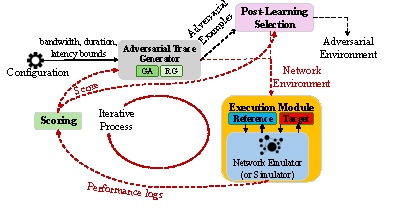
\includegraphics[width=81mm,height=45mm,keepaspectratio]{architecture.pdf}
\end{textblock*}
\end{frame}
\note{AdvNet addresses these gaps by formulating environment generation as a black-box search over real protocol executions. The user provides parameter bounds, a \textbf{target} protocol under test, and a \textbf{reference} baseline—which can be another protocol, an older version of the same protocol, a single-path configuration, or a calculated capacity benchmark.
\par\smallskip Source: AdvNet paper Fig.1; §3}


% Slide 9: The performance-gap score
% AdvNet paper §3.5, Eq.(1)
\begin{frame}[plain]
\begin{textblock*}{144mm}(8mm,6mm)
\raggedright\color[HTML]{142D45}\fontsize{22}{27.06}\selectfont \bfseries The performance-gap score
\end{textblock*}
\begin{textblock*}{70mm}(8mm,23mm)
\raggedright\color[HTML]{142D45}\fontsize{16}{19.68}\selectfont \(\displaystyle \mathrm{score}=\frac{R-P}{\max(R,P)}\)
\end{textblock*}
\begin{textblock*}{67mm}(85mm,25mm)
\raggedright\color[HTML]{142D45}\fontsize{10.5}{12.915}\selectfont Higher is better: R = reference, P = target\par Example: R = 10, P = 2 gives score = 0.8
\end{textblock*}
\begin{textblock*}{144mm}(8mm,45mm)
\raggedright\color[HTML]{142D45}\fontsize{16}{19.68}\selectfont \(\displaystyle U=t_{\mathrm{coeff}}\frac{\tau}{\tau_{\max}}+(1-t_{\mathrm{coeff}})\frac{d_{\min}}{d}\)
\end{textblock*}
\begin{textblock*}{144mm}(8mm,65mm)
\raggedright\color[HTML]{526474}\fontsize{9.3}{11.439}\selectfont τ: throughput; d: average packet delay; τmax and dmin: normalization benchmarks
\end{textblock*}
\begin{textblock*}{144mm}(8mm,76mm)
\raggedright\color[HTML]{2869B3}\fontsize{9.2}{11.316}\selectfont Throughput weight: 0 = delay only, 0.5 = equal normalized weights, 1 = throughput only
\end{textblock*}
\end{frame}
\note{In each iteration, the generator outputs a candidate network trace, and the execution module runs the target and, when the reference is another protocol, runs the reference inside an extended Mahimahi emulator (which the authors modified to support time-varying one-way delay and dual paths). The scoring module then quantifies their relative performance gap as a \textbf{score}:\par \par \[
\text{score} = \frac{R - P}{\max(R, P)} \quad (\text{when higher metric is better}).
\]\par \par For example, if the reference achieves $R = 10$ Mbps and the target gets only $P = 2$ Mbps, the score is $(10 - 2)/10 = 0.8$. If a lower metric is better—such as flow completion time—we reverse the numerator to $P - R$. For nonnegative metrics with a positive denominator, dividing by the maximum normalizes the score between $-1$ and $1$, so a larger positive score always means a larger relative weakness in the target. We can also combine throughput $\tau$ and average packet delay $d$ into a single utility metric using a throughput weight $t_{\mathrm{coeff}} \in [0, 1]$:\par \par \[
U = t_{\mathrm{coeff}} \frac{\tau}{\tau_{\max}} + (1 - t_{\mathrm{coeff}}) \frac{d_{\min}}{d},
\]\par \par where $t_{\mathrm{coeff}} = 1$ cares only about throughput, $0$ cares only about delay, and $0.5$ weights the two normalized terms equally. Here, $\tau_{\max}$ and $d_{\min}$ are the throughput and delay normalization benchmarks.
\par\smallskip Source: AdvNet paper §3.5, Eq.(1)}


% Slide 10: Post-learning selection
% AdvNet paper §1–3
\begin{frame}[plain]
\begin{textblock*}{144mm}(8mm,6mm)
\raggedright\color[HTML]{142D45}\fontsize{22}{27.06}\selectfont \bfseries Post-learning selection
\end{textblock*}
\begin{textblock*}{43mm}(8mm,27mm)
\raggedright\color[HTML]{2869B3}\fontsize{12}{14.76}\selectfont \bfseries Search
\end{textblock*}
\begin{textblock*}{43mm}(8mm,41mm)
\raggedright\color[HTML]{142D45}\fontsize{13}{15.99}\selectfont Generate and evaluate new candidate traces
\end{textblock*}
\begin{textblock*}{43mm}(59mm,27mm)
\raggedright\color[HTML]{087F82}\fontsize{12}{14.76}\selectfont \bfseries PLS
\end{textblock*}
\begin{textblock*}{43mm}(59mm,41mm)
\raggedright\color[HTML]{142D45}\fontsize{13}{15.99}\selectfont Re-measure promising candidates and select by mean
\end{textblock*}
\begin{textblock*}{42mm}(110mm,27mm)
\raggedright\color[HTML]{C06821}\fontsize{12}{14.76}\selectfont \bfseries Independent check
\end{textblock*}
\begin{textblock*}{42mm}(110mm,41mm)
\raggedright\color[HTML]{142D45}\fontsize{13}{15.99}\selectfont Re-evaluate the returned trace
\end{textblock*}
\end{frame}
\note{Finally, because emulation has random variance, AdvNet reserves the last portion of its time budget for \textbf{Post-Learning Selection (PLS)} to choose among promising candidates using repeated measurements and observed mean scores, followed by an independent re-evaluation.
\par\smallskip Source: AdvNet paper §1–3}


% Slide 11: Two design challenges
% AdvNet paper §1–3
\begin{frame}[plain]
\begin{textblock*}{144mm}(8mm,6mm)
\raggedright\color[HTML]{142D45}\fontsize{22}{27.06}\selectfont \bfseries Two design challenges
\end{textblock*}
\begin{textblock*}{144mm}(8mm,22mm)
\raggedright\color[HTML]{2869B3}\fontsize{11.5}{14.145}\selectfont The framework must find useful failures within a limited budget.
\end{textblock*}
\begin{textblock*}{68mm}(8mm,34mm)
\raggedright\color[HTML]{2869B3}\fontsize{12}{14.76}\selectfont \bfseries Sample efficiency
\end{textblock*}
\begin{textblock*}{68mm}(8mm,45mm)
\raggedright\color[HTML]{142D45}\fontsize{11.5}{14.145}\selectfont \begin{itemize}\setlength{\itemsep}{2.6mm}\setlength{\parskip}{0pt}
\item Real-code runs cost time
\item Large environment space
\item Repetition competes with exploration
\end{itemize}
\end{textblock*}
\begin{textblock*}{67mm}(85mm,34mm)
\raggedright\color[HTML]{087F82}\fontsize{12}{14.76}\selectfont \bfseries Practical usefulness
\end{textblock*}
\begin{textblock*}{67mm}(85mm,45mm)
\raggedright\color[HTML]{142D45}\fontsize{11.5}{14.145}\selectfont \begin{itemize}\setlength{\itemsep}{2.6mm}\setlength{\parskip}{0pt}
\item Avoid trivial zero-capacity examples
\item Allow expected adaptation delays
\item Choose meaningful reference comparisons
\end{itemize}
\end{textblock*}
\end{frame}
\note{Realizing this framework in emulation brings two main challenges:\par \par The first challenge is \textbf{sample efficiency}. Because every evaluation runs real kernel protocols over emulated links for several seconds, we can only afford a limited number of runs. Meanwhile, the space of time-varying parameters is huge, and emulation noise means a single run can be misleading—yet repeating every trace many times would leave very little budget to explore new environments.\par \par The second challenge is \textbf{practical usefulness}. Setting link bandwidth to zero makes every protocol get zero throughput, which is useless for diagnosis. Similarly, if bandwidth jumps instantaneously, any protocol needs time to adapt, so falling short of link capacity right after a spike is expected. Using a realistic reference—and designing the comparison around concrete developer tasks—is essential to uncover actionable flaws.
\par\smallskip Source: AdvNet paper §1–3}


% Slide 12: Representing a network trace
% AdvNet paper §3.1, Table 1; teaching example
\begin{frame}[plain]
\begin{textblock*}{144mm}(8mm,6mm)
\raggedright\color[HTML]{142D45}\fontsize{22}{27.06}\selectfont \bfseries Representing a network trace
\end{textblock*}
\begin{textblock*}{92mm}(8mm,23mm)
\raggedright\color[HTML]{2869B3}\fontsize{11.5}{14.145}\selectfont First, keep the environment search space compact.
\end{textblock*}
\begin{textblock*}{42mm}(110mm,24mm)
\raggedright\color[HTML]{142D45}\fontsize{15}{18.45}\selectfont \(\displaystyle T=(B,L,D,I)\)
\end{textblock*}
\begin{textblock*}{144mm}(8mm,37mm)
\raggedright\color[HTML]{142D45}\fontsize{10.5}{12.915}\selectfont \setlength{\tabcolsep}{1.4mm}\renewcommand{\arraystretch}{1.35}
\begin{tabular}{@{}>{\raggedright\arraybackslash}p{23.052mm}>{\raggedright\arraybackslash}p{37.968mm}>{\raggedright\arraybackslash}p{42.036mm}>{\raggedright\arraybackslash}p{32.544mm}@{}}\toprule
\textbf{Interval} & \textbf{B: bandwidth} & \textbf{L: one-way delay} & \textbf{D: duration}\\
\midrule
1 & 20 Mbps & 20 ms & 1 s\\
2 & 5 Mbps & 80 ms & 2 s\\
3 & 20 Mbps & 10 ms & 1 s\\
\bottomrule\end{tabular}
\end{textblock*}
\begin{textblock*}{144mm}(8mm,72mm)
\raggedright\color[HTML]{142D45}\fontsize{10}{12.3}\selectfont I: queue capacity and optional transfer size, fixed within a trace
\end{textblock*}
\begin{textblock*}{144mm}(8mm,81mm)
\raggedright\color[HTML]{526474}\fontsize{9.5}{11.685}\selectfont Table 1 bounds: 1–100 Mbps, 5–100 ms, 0.5–2.5 s per interval
\end{textblock*}
\end{frame}
\note{Now, what exactly does the search change? AdvNet represents a trace using four parts:\par \par \[
T=(B,L,D,I).
\]\par \par $B$ contains bandwidths, $L$ contains one-way delays, and $D$ contains interval durations. $I$ contains parameters that stay fixed within the trace, such as queue capacity. For multipath tests, each link has its own bandwidth and delay sequence, with shared interval durations.\par \par Here is a teaching example. The first interval has twenty megabits per second and twenty milliseconds of one-way delay. Bandwidth then falls while delay rises. Finally, bandwidth recovers and delay falls. Each parameter is constrained within user-specified bounds (for example, 1 to 100 Mbps, 5 to 100 ms, and 0.5 to 2.5 seconds per interval in Table 1).
\par\smallskip Source: AdvNet paper §3.1, Table 1; teaching example}


% Slide 13: Intervals versus packet delivery opportunities
% AdvNet paper §4.2.1, Table 2
\begin{frame}[plain]
\begin{textblock*}{144mm}(8mm,6mm)
\raggedright\color[HTML]{142D45}\fontsize{18.7}{23.001}\selectfont \bfseries Intervals versus packet delivery opportunities
\end{textblock*}
\begin{textblock*}{81mm}(8mm,27mm)
\raggedright\color[HTML]{142D45}\fontsize{11}{13.53}\selectfont \setlength{\tabcolsep}{1.4mm}\renewcommand{\arraystretch}{1.35}
\begin{tabular}{@{}>{\raggedright\arraybackslash}p{22.620mm}>{\raggedright\arraybackslash}p{26.390mm}>{\raggedright\arraybackslash}p{26.390mm}@{}}\toprule
\textbf{Target} & \textbf{Intervals} & \textbf{PDOs}\\
\midrule
BBR & 79.11\% & 14.31\%\\
CUBIC & 46.24\% & 29.78\%\\
Vegas & 84.71\% & 27.29\%\\
Reno & 41.26\% & 28.80\%\\
\bottomrule\end{tabular}
\end{textblock*}
\begin{textblock*}{54mm}(98mm,26mm)
\raggedright\color[HTML]{142D45}\fontsize{11}{13.53}\selectfont \begin{itemize}\setlength{\itemsep}{2.6mm}\setlength{\parskip}{0pt}
\item Matched comparison inside AdvNet
\item Higher PDO dimension makes search harder
\item Direct control of delay changes
\end{itemize}
\end{textblock*}
\begin{textblock*}{144mm}(8mm,79mm)
\raggedright\color[HTML]{526474}\fontsize{9.3}{11.439}\selectfont Higher scores expose larger throughput shortfalls. This compares representations, not complete systems.
\end{textblock*}
\end{frame}
\note{Why use intervals instead of CC-Fuzz's packet delivery opportunities (PDOs), where each PDO specifies the exact timestamp when a packet can leave? The authors implemented the PDO representation inside AdvNet and compared both under matched genetic algorithm settings and a one-hour budget (Table 2). Across all four protocols, AdvNet's interval representation achieves much higher scores—for instance, about 79\% versus 14\% on BBR.\par \par The authors point to two reasons. First, PDOs create a much higher-dimensional search space: when the number of PDOs is increased from 25 to 100, the search struggles even more, and the score on BBR drops from 14.31\% down to 5.91\%. Second, AdvNet directly exposes link delay changes as tunable parameters, which turns out to be critical for triggering several protocol bugs.
\par\smallskip Source: AdvNet paper §4.2.1, Table 2}


% Slide 14: Trace-based and action-based adversaries
% AdvNet paper §1–3
\begin{frame}[plain]
\begin{textblock*}{144mm}(8mm,6mm)
\raggedright\color[HTML]{142D45}\fontsize{20}{24.6}\selectfont \bfseries Trace-based and action-based adversaries
\end{textblock*}
\begin{textblock*}{144mm}(8mm,22mm)
\raggedright\color[HTML]{2869B3}\fontsize{11.5}{14.145}\selectfont We have a trace representation. How should the search use it?
\end{textblock*}
\begin{textblock*}{68mm}(8mm,34mm)
\raggedright\color[HTML]{2869B3}\fontsize{12}{14.76}\selectfont \bfseries Action-based adversary
\end{textblock*}
\begin{textblock*}{68mm}(8mm,45mm)
\raggedright\color[HTML]{142D45}\fontsize{11.5}{14.145}\selectfont \begin{itemize}\setlength{\itemsep}{2.6mm}\setlength{\parskip}{0pt}
\item Observe state and choose the next condition online
\item Requires reliable synchronization despite scheduling jitter
\end{itemize}
\end{textblock*}
\begin{textblock*}{67mm}(85mm,34mm)
\raggedright\color[HTML]{087F82}\fontsize{12}{14.76}\selectfont \bfseries Trace-based adversary
\end{textblock*}
\begin{textblock*}{67mm}(85mm,45mm)
\raggedright\color[HTML]{142D45}\fontsize{11.5}{14.145}\selectfont \begin{itemize}\setlength{\itemsep}{2.6mm}\setlength{\parskip}{0pt}
\item Generate the full trace before execution
\item Replay the same external conditions for comparison
\end{itemize}
\end{textblock*}
\end{frame}
\note{With the representation fixed, how does AdvNet search for challenging environments?\par \par The authors first considered an \textbf{action-based} online adversary, such as reinforcement learning, that observes protocol state and chooses the next network condition on the fly. However, when running both a target and a reference in emulation, their internal states naturally diverge, and OS scheduling jitter makes it difficult to keep online actions synchronized across both runs. They therefore chose a \textbf{trace-based} adversary that outputs a complete trace before execution, making external conditions easier to replay and compare without online action synchronization.
\par\smallskip Source: AdvNet paper §1–3}


% Slide 15: Genetic algorithms in AdvNet
% AdvNet paper §1–3
\begin{frame}[plain]
\begin{textblock*}{144mm}(8mm,6mm)
\raggedright\color[HTML]{142D45}\fontsize{22}{27.06}\selectfont \bfseries Genetic algorithms in AdvNet
\end{textblock*}
\begin{textblock*}{47mm}(8mm,26mm)
\raggedright\color[HTML]{2869B3}\fontsize{12}{14.76}\selectfont \bfseries Select
\end{textblock*}
\begin{textblock*}{47mm}(8mm,37mm)
\raggedright\color[HTML]{142D45}\fontsize{11.5}{14.145}\selectfont Favor promising traces
\end{textblock*}
\begin{textblock*}{47mm}(8mm,51mm)
\raggedright\color[HTML]{087F82}\fontsize{12}{14.76}\selectfont \bfseries Recombine
\end{textblock*}
\begin{textblock*}{47mm}(8mm,62mm)
\raggedright\color[HTML]{142D45}\fontsize{11.5}{14.145}\selectfont Exchange parameter segments
\end{textblock*}
\begin{textblock*}{92mm}(60mm,34mm)
\raggedright\color[HTML]{142D45}\fontsize{11}{13.53}\selectfont 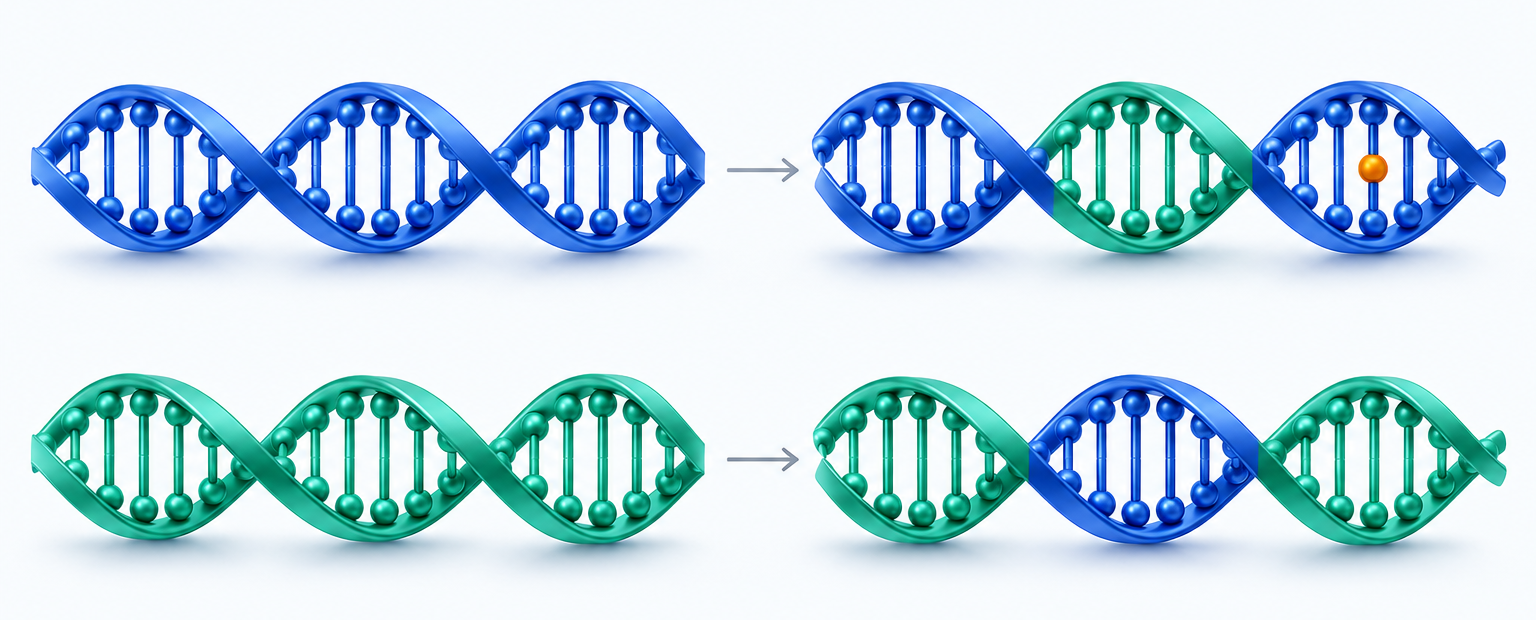
\includegraphics[width=92mm,height=39mm,keepaspectratio]{ga-dna.png}
\end{textblock*}
\begin{textblock*}{92mm}(60mm,24mm)
\raggedright\color[HTML]{142D45}\fontsize{10.5}{12.915}\selectfont Candidate = a complete trace\par Fitness = measured performance-gap score
\end{textblock*}
\begin{textblock*}{92mm}(60mm,78mm)
\raggedright\color[HTML]{C06821}\fontsize{9.7}{11.931}\selectfont Mutation introduces new values; every child still needs evaluation.
\end{textblock*}
\end{frame}
\note{AdvNet's main search method is a \textbf{genetic algorithm (GA)}. Each candidate is a complete network trace, and its genes are the numerical parameters in $T$. GA maintains a population of traces, evaluates their fitness using the performance-gap score, selects promising parents, and applies crossover and mutation to produce the next generation until the budget expires.
\par\smallskip Source: AdvNet paper §1–3}


% Slide 16: Crossover and integer mutation
% AdvNet paper §1–3
\begin{frame}[plain]
\begin{textblock*}{144mm}(8mm,6mm)
\raggedright\color[HTML]{142D45}\fontsize{22}{27.06}\selectfont \bfseries Crossover and integer mutation
\end{textblock*}
\begin{textblock*}{87mm}(8mm,24mm)
\raggedright\color[HTML]{2869B3}\fontsize{12}{14.76}\selectfont \bfseries Two-point crossover
\end{textblock*}
\begin{textblock*}{87mm}(8mm,36mm)
\raggedright\color[HTML]{142D45}\fontsize{10.2}{12.546}\selectfont \setlength{\tabcolsep}{1.4mm}\renewcommand{\arraystretch}{1.35}
\begin{tabular}{@{}>{\raggedright\arraybackslash}p{27.288mm}>{\raggedright\arraybackslash}p{12.128mm}>{\raggedright\arraybackslash}p{12.128mm}>{\raggedright\arraybackslash}p{12.128mm}>{\raggedright\arraybackslash}p{12.128mm}@{}}\toprule
\textbf{} & \textbf{x\(_1\)} & \textbf{x\(_2\)} & \textbf{x\(_3\)} & \textbf{x\(_4\)}\\
\midrule
Parent A & \cellcolor{paleblue}20 & \cellcolor{paleblue}5 & \cellcolor{paleblue}40 & \cellcolor{paleblue}10\\
Parent B & \cellcolor{paleteal}60 & \cellcolor{paleteal}30 & \cellcolor{paleteal}15 & \cellcolor{paleteal}80\\
Child 1 & \cellcolor{paleblue}20 & \cellcolor{paleteal}30 & \cellcolor{paleteal}15 & \cellcolor{paleblue}10\\
Child 2 & \cellcolor{paleteal}60 & \cellcolor{paleblue}5 & \cellcolor{paleblue}40 & \cellcolor{paleteal}80\\
\bottomrule\end{tabular}
\end{textblock*}
\begin{textblock*}{48mm}(104mm,24mm)
\raggedright\color[HTML]{087F82}\fontsize{12}{14.76}\selectfont \bfseries Integer mutation
\end{textblock*}
\begin{textblock*}{48mm}(104mm,38mm)
\raggedright\color[HTML]{142D45}\fontsize{11}{13.53}\selectfont Each gene mutates\par with probability p.
\end{textblock*}
\begin{textblock*}{48mm}(104mm,59mm)
\raggedright\color[HTML]{C06821}\fontsize{21}{25.83}\selectfont \bfseries 15 → 73
\end{textblock*}
\begin{textblock*}{48mm}(104mm,74mm)
\raggedright\color[HTML]{526474}\fontsize{9.5}{11.685}\selectfont Sample from that gene’s allowed range.\par Toy range here: 1–100.
\end{textblock*}
\end{frame}
\note{Let us look at the two operators. In \textbf{two-point crossover}, we choose two cut points and swap the middle segment between two parent traces. In a four-gene example, each child keeps one parent's outer values and takes the other parent's middle values. In real traces, because crossover swaps aligned positions, a bandwidth parameter always replaces a bandwidth parameter, preserving each gene's allowed bounds.\par \par \textbf{Uniform integer mutation} replaces each gene with probability $p$ by sampling a new integer uniformly from that gene's allowed range—for example, changing 15 to 73. Both operators preserve the integer format required by Mahimahi, and every newly generated trace is evaluated by running the protocols.
\par\smallskip Source: AdvNet paper §1–3}


% Slide 17: Evidence for the search design
% AdvNet paper §4.2.3, Fig.3
\begin{frame}[plain]
\begin{textblock*}{144mm}(8mm,6mm)
\raggedright\color[HTML]{142D45}\fontsize{22}{27.06}\selectfont \bfseries Evidence for the search design
\end{textblock*}
\begin{textblock*}{69mm}(8mm,24mm)
\raggedright\color[HTML]{2869B3}\fontsize{12}{14.76}\selectfont \bfseries GA versus random generation\par \normalfont\fontsize{9.7}{11.931}\selectfont 1 hour total; 6 min PLS when enabled
\end{textblock*}
\begin{textblock*}{67mm}(85mm,24mm)
\raggedright\color[HTML]{087F82}\fontsize{12}{14.76}\selectfont \bfseries GA, BO, and EPS\par \normalfont\fontsize{9.7}{11.931}\selectfont 2 hours total; last 12 min for PLS
\end{textblock*}
\begin{textblock*}{69mm}(8mm,36mm)
\raggedright\color[HTML]{142D45}\fontsize{11}{13.53}\selectfont 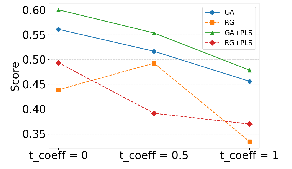
\includegraphics[width=69mm,height=36mm,keepaspectratio]{optimizers-random.pdf}
\end{textblock*}
\begin{textblock*}{67mm}(85mm,36mm)
\raggedright\color[HTML]{142D45}\fontsize{11}{13.53}\selectfont 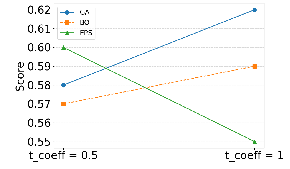
\includegraphics[width=67mm,height=36mm,keepaspectratio]{optimizers-active.pdf}
\end{textblock*}
\begin{textblock*}{144mm}(8mm,77mm)
\raggedright\color[HTML]{087F82}\fontsize{11.5}{14.145}\selectfont High scores are promising. Final selection still has to handle noise.
\end{textblock*}
\end{frame}
\note{The authors also compared GA against three other trace-based methods: \textbf{Random Generation (RG)}, which samples traces uniformly at random as a baseline; \textbf{Bayesian Optimization (BO)} with a random forest surrogate model; and \textbf{Epsilon-Greedy Search (EPS)}, which mutates top-performing traces with probability $1-\epsilon$ and explores randomly with probability $\epsilon$.\par \par In Figure 3a, under a one-hour budget across 20 protocol pairs, GA consistently outperforms random generation across all three throughput weights $t_{\mathrm{coeff}} = 0, 0.5,$ and $1$ (improving scores by 23\% on average), supporting the benefit of using execution feedback under these tested settings. In Figure 3b, under a two-hour budget, GA, Bayesian optimization, and epsilon-greedy search achieve fairly similar performance, with GA having a slightly higher average, so the authors adopt GA as the default.
\par\smallskip Source: AdvNet paper §4.2.3, Fig.3}


% Slide 18: Noisy scores and SimpleMax
% AdvNet paper §1–3
\begin{frame}[plain]
\begin{textblock*}{144mm}(8mm,6mm)
\raggedright\color[HTML]{142D45}\fontsize{22}{27.06}\selectfont \bfseries Noisy scores and SimpleMax
\end{textblock*}
\begin{textblock*}{144mm}(8mm,22mm)
\raggedright\color[HTML]{2869B3}\fontsize{11.5}{14.145}\selectfont The search returns many candidates. Which trace should we keep?
\end{textblock*}
\begin{textblock*}{144mm}(8mm,36mm)
\raggedright\color[HTML]{2869B3}\fontsize{12}{14.76}\selectfont \bfseries SimpleMax
\end{textblock*}
\begin{textblock*}{144mm}(8mm,48mm)
\raggedright\color[HTML]{142D45}\fontsize{13}{15.99}\selectfont Keep the trace with the largest score observed during search.
\end{textblock*}
\begin{textblock*}{144mm}(8mm,63mm)
\raggedright\color[HTML]{142D45}\fontsize{12}{14.76}\selectfont \begin{itemize}\setlength{\itemsep}{2.6mm}\setlength{\parskip}{0pt}
\item Hundreds of candidates create chances for lucky observations
\item The apparent winner may score lower when re-tested
\end{itemize}
\end{textblock*}
\end{frame}
\note{Finding high scores during search is only part of the problem; measurement noise can still mislead our final choice. The simplest rule, \textbf{SimpleMax}, simply outputs whichever trace had the single highest observed score during search.\par \par However, when evaluating hundreds of traces, the single highest observation is often a "lucky outlier" inflated by positive random noise, whose score drops sharply when re-tested independently.
\par\smallskip Source: AdvNet paper §1–3}


% Slide 19: Multi-round elimination
% AdvNet paper §1–3
\begin{frame}[plain]
\begin{textblock*}{144mm}(8mm,6mm)
\raggedright\color[HTML]{142D45}\fontsize{22}{27.06}\selectfont \bfseries Multi-round elimination
\end{textblock*}
\begin{textblock*}{144mm}(8mm,22mm)
\raggedright\color[HTML]{2869B3}\fontsize{11.5}{14.145}\selectfont PLS spends extra evaluations on the most promising candidates.
\end{textblock*}
\begin{textblock*}{35mm}(8mm,34mm)
\raggedright\color[HTML]{2869B3}\fontsize{35}{43.05}\selectfont \bfseries 25
\end{textblock*}
\begin{textblock*}{45mm}(8mm,57mm)
\raggedright\color[HTML]{142D45}\fontsize{12}{14.76}\selectfont Top search candidates
\end{textblock*}
\begin{textblock*}{91mm}(61mm,35mm)
\raggedright\color[HTML]{142D45}\fontsize{11.5}{14.145}\selectfont \begin{itemize}\setlength{\itemsep}{2.6mm}\setlength{\parskip}{0pt}
\item Evaluate every remaining candidate once
\item Remove roughly the lower half by observed mean
\item At five or fewer, keep measuring until the budget ends
\item Return the highest observed mean
\end{itemize}
\end{textblock*}
\end{frame}
\note{To mitigate noise, AdvNet runs each trace multiple times in parallel during search and uses the \textbf{median reference and target performance measurements} to compute the score. After search finishes, \textbf{Post-Learning Selection (PLS)} takes the top 25 candidate environments and allocates a dedicated evaluation budget using \textbf{Multi-Round Elimination (MRE)}. In each round, MRE evaluates every remaining candidate once and discards roughly the lower half based on their observed mean scores so far. Once 5 or fewer candidates remain, elimination stops and they are repeatedly evaluated until the budget is spent, returning the one with the highest mean score (which is then checked in one final independent evaluation).
\par\smallskip Source: AdvNet paper §1–3}


% Slide 20: The search and selection budget
% AdvNet paper §4.2.2, Fig.2
\begin{frame}[plain]
\begin{textblock*}{144mm}(8mm,6mm)
\raggedright\color[HTML]{142D45}\fontsize{22}{27.06}\selectfont \bfseries The search and selection budget
\end{textblock*}
\begin{textblock*}{76mm}(8mm,27mm)
\raggedright\color[HTML]{142D45}\fontsize{11}{13.53}\selectfont 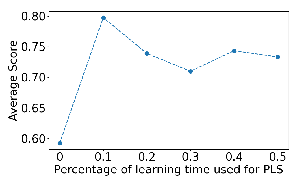
\includegraphics[width=76mm,height=49mm,keepaspectratio]{pls-budget.pdf}
\end{textblock*}
\begin{textblock*}{58mm}(94mm,27mm)
\raggedright\color[HTML]{087F82}\fontsize{24}{29.52}\selectfont \bfseries 90\% search\par 10\% PLS
\end{textblock*}
\begin{textblock*}{58mm}(94mm,61mm)
\raggedright\color[HTML]{142D45}\fontsize{10.5}{12.915}\selectfont \begin{itemize}\setlength{\itemsep}{2.6mm}\setlength{\parskip}{0pt}
\item Best split in this experiment
\item More selection means less exploration
\end{itemize}
\end{textblock*}
\end{frame}
\note{How should we split the total runtime between search and PLS? In Figure 2, when $0\%$ of the time is used for PLS (which is just SimpleMax), noisy outliers leave the average re-tested score around $0.59$. Dedicating **$10\%$** of the runtime to PLS (and $90\%$ to GA search) raises the average score to about $0.80$, an increase of roughly $0.21$ score units. Spending more than $10\%$ on PLS causes the score to dip slightly, because taking too much time away from GA leaves fewer iterations to discover strong candidates in the first place.
\par\smallskip Source: AdvNet paper §4.2.2, Fig.2}


% Slide 21: From search design to practical use
% AdvNet paper §1–3
\begin{frame}[plain]
\begin{textblock*}{144mm}(8mm,6mm)
\raggedright\color[HTML]{142D45}\fontsize{22}{27.06}\selectfont \bfseries From search design to practical use
\end{textblock*}
\begin{textblock*}{144mm}(8mm,27mm)
\raggedright\color[HTML]{142D45}\fontsize{13}{15.99}\selectfont \begin{itemize}\setlength{\itemsep}{2.6mm}\setlength{\parskip}{0pt}
\item Compact representation makes the search manageable
\item GA uses execution feedback to discover challenging traces
\item PLS selects an output for practical investigation
\end{itemize}
\end{textblock*}
\begin{textblock*}{144mm}(8mm,77mm)
\raggedright\color[HTML]{087F82}\fontsize{12}{14.76}\selectfont \bfseries Next: Xiaoyang presents the protocol testing use cases.
\end{textblock*}
\end{frame}
\note{Together, the compact interval representation, genetic search, and post-learning selection allow AdvNet to find reliably adversarial environments within a limited emulation budget. With that, I will hand over to Xiaoyang, who will show how AdvNet uses these environments across concrete protocol testing use cases.
\par\smallskip Source: AdvNet paper §1–3}


% Slide 22: Developer tasks and comparisons
% AdvNet paper §1–3
\begin{frame}[plain]
\begin{textblock*}{144mm}(8mm,6mm)
\raggedright\color[HTML]{142D45}\fontsize{22}{27.06}\selectfont \bfseries Developer tasks and comparisons
\end{textblock*}
\begin{textblock*}{144mm}(8mm,25mm)
\raggedright\color[HTML]{142D45}\fontsize{9.5}{11.685}\selectfont \setlength{\tabcolsep}{1.4mm}\renewcommand{\arraystretch}{1.35}
\begin{tabular}{@{}>{\raggedright\arraybackslash}p{16.272mm}>{\raggedright\arraybackslash}p{42.036mm}>{\raggedright\arraybackslash}p{46.104mm}>{\raggedright\arraybackslash}p{31.188mm}@{}}\toprule
\textbf{Use case} & \textbf{Reference} & \textbf{Target / comparison} & \textbf{Question}\\
\midrule
UC1 & Capacity, another TCP, or a reference flow alone & Protocol under test, or reference with a competitor & Underutilization or unfairness?\\
UC2 & Earlier protocol version & Newer version; compare the same metric & Did an update regress?\\
UC3 & One path & Two paths & Can an extra path hurt?\\
\bottomrule\end{tabular}
\end{textblock*}
\end{frame}
\note{Now that we have seen how AdvNet searches efficiently, let's look at how developers can use it to answer practical questions. By simply changing how we define the \textbf{reference} and the \textbf{target} inside the same scoring pipeline, the authors apply AdvNet to three distinct use cases:\par \par * \textbf{UC1 — Finding suboptimal performance and fairness issues}: We set the target to be the protocol under test, and compare it against either theoretical link capacity or another protocol implementation (or compare a reference flow running alone versus competing head-to-head with the target) to uncover severe underutilization, kernel bugs, or starvation.\par * \textbf{UC2 — Regression testing across versions}: We set the older version of a protocol as the reference and the newer version as the target, searching for environments where an update degrades throughput or fairness.\par * \textbf{UC3 — Validating design objectives}: To test the "do no harm" goal of multipath transport, we set a single-path configuration as the reference and a dual-path configuration as the target.\par \par Let's examine what AdvNet discovered in each of these three use cases.
\par\smallskip Source: AdvNet paper §1–3}


% Slide 23: 17 TCP protocols: pairwise robustness
% AdvNet paper §4.3, Fig.4(a)
\begin{frame}[plain]
\begin{textblock*}{144mm}(8mm,6mm)
\raggedright\color[HTML]{142D45}\fontsize{22}{27.06}\selectfont \bfseries 17 TCP protocols: pairwise robustness
\end{textblock*}
\begin{textblock*}{72mm}(8mm,22mm)
\raggedright\color[HTML]{142D45}\fontsize{11}{13.53}\selectfont 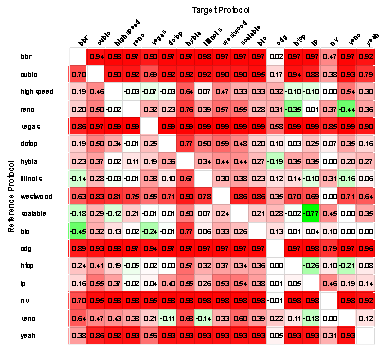
\includegraphics[width=72mm,height=64mm,keepaspectratio]{matrix-balanced.pdf}
\end{textblock*}
\begin{textblock*}{66mm}(86mm,24mm)
\raggedright\color[HTML]{2869B3}\fontsize{12}{14.76}\selectfont \bfseries Equal throughput / delay weights
\end{textblock*}
\begin{textblock*}{66mm}(86mm,36mm)
\raggedright\color[HTML]{142D45}\fontsize{10.5}{12.915}\selectfont 17 protocols\par 272 directed pairs per objective\par 544 scenarios across both objectives
\end{textblock*}
\begin{textblock*}{66mm}(86mm,65mm)
\raggedright\color[HTML]{2869B3}\fontsize{23}{28.29}\selectfont \bfseries 448 / 544
\end{textblock*}
\begin{textblock*}{66mm}(86mm,80mm)
\raggedright\color[HTML]{526474}\fontsize{9.7}{11.931}\selectfont scenarios with a positive score
\end{textblock*}
\end{frame}
\note{Under UC1, while comparing against theoretical link capacity can flag extreme underutilization, comparing against another real protocol is even more informative: if another protocol achieves much higher performance under the exact same trace, we know better performance is achievable in practice.\par \par The authors ran an all-pairs comparison across 17 TCP congestion control algorithms in the Linux kernel (Figure 4). That gives $17\times16=272$ directed pairs, tested under two utility definitions—an equal 50/50 split between throughput and delay ($t_{\mathrm{coeff}}=0.5$), and throughput only ($t_{\mathrm{coeff}}=1$)—for 544 scenarios in total, each with a two-hour budget. AdvNet found adversarial environments (positive scores) in 448 of the 544 scenarios, and every single protocol had at least one environment where another reference protocol substantially outperformed it.
\par\smallskip Source: AdvNet paper §4.3, Fig.4(a)}


% Slide 24: Different traces, different weaknesses
% AdvNet paper §4.3, Fig.4(b)
\begin{frame}[plain]
\begin{textblock*}{144mm}(8mm,6mm)
\raggedright\color[HTML]{142D45}\fontsize{22}{27.06}\selectfont \bfseries Different traces, different weaknesses
\end{textblock*}
\begin{textblock*}{72mm}(8mm,22mm)
\raggedright\color[HTML]{142D45}\fontsize{11}{13.53}\selectfont 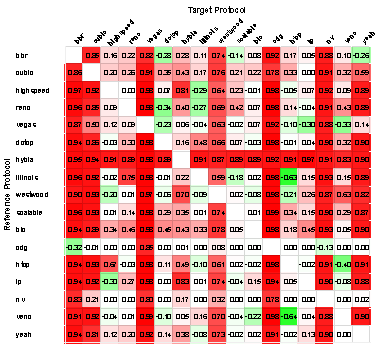
\includegraphics[width=72mm,height=64mm,keepaspectratio]{matrix-throughput.pdf}
\end{textblock*}
\begin{textblock*}{66mm}(86mm,24mm)
\raggedright\color[HTML]{2869B3}\fontsize{12}{14.76}\selectfont \bfseries Throughput-only objective
\end{textblock*}
\begin{textblock*}{66mm}(86mm,38mm)
\raggedright\color[HTML]{142D45}\fontsize{10}{12.3}\selectfont \setlength{\tabcolsep}{1.4mm}\renewcommand{\arraystretch}{1.35}
\begin{tabular}{@{}>{\raggedright\arraybackslash}p{21.744mm}>{\raggedright\arraybackslash}p{21.744mm}>{\raggedright\arraybackslash}p{16.912mm}@{}}\toprule
\textbf{Reference} & \textbf{Target} & \textbf{Score}\\
\midrule
BBR & CUBIC & 0.85\\
CUBIC & BBR & 0.86\\
\bottomrule\end{tabular}
\end{textblock*}
\begin{textblock*}{66mm}(86mm,69mm)
\raggedright\color[HTML]{C06821}\fontsize{11}{13.53}\selectfont Each cell uses a different discovered trace. Both directions can reveal a weakness.
\end{textblock*}
\end{frame}
\note{Look at BBR and CUBIC in the top-left corner of both heatmaps. Under both objectives, whether BBR is the reference and CUBIC is the target (scores of $0.94$ and $0.85$), or CUBIC is the reference and BBR is the target (scores of $0.70$ and $0.86$), AdvNet finds environments with large performance gaps in both directions. Because each cell comes from a separate search, this is not a contradiction: it shows that even under the same metric, both protocols have distinct blind spots under different network dynamics.\par \par However, a high score alone only tells us *where* a protocol struggles, not *why*. Next, let's look at how the authors diagnosed the root causes inside several discovered environments.
\par\smallskip Source: AdvNet paper §4.3, Fig.4(b)}


% Slide 25: A Linux TCP acknowledgment bug
% AdvNet paper §4.4.1
\begin{frame}[plain]
\begin{textblock*}{144mm}(8mm,6mm)
\raggedright\color[HTML]{142D45}\fontsize{22}{27.06}\selectfont \bfseries A Linux TCP acknowledgment bug
\end{textblock*}
\begin{textblock*}{144mm}(8mm,25mm)
\raggedright\color[HTML]{142D45}\fontsize{10.6}{13.038}\selectfont \setlength{\tabcolsep}{1.4mm}\renewcommand{\arraystretch}{1.35}
\begin{tabular}{@{}>{\raggedright\arraybackslash}p{14.120mm}>{\raggedright\arraybackslash}p{127.080mm}@{}}\toprule
\textbf{Step} & \textbf{Observed event}\\
\midrule
1 & Delay drops; later packets arrive first\\
2 & Three duplicate ACKs trigger fast retransmit\\
3 & The original packet arrives before its retransmission\\
4 & ACK advancement fails; duplicate ACKs persist\\
5 & The sender enters retransmission timeout\\
\bottomrule\end{tabular}
\end{textblock*}
\begin{textblock*}{144mm}(8mm,81mm)
\raggedright\color[HTML]{526474}\fontsize{9.5}{11.685}\selectfont eBPF and Wireshark helped the authors diagnose the packet sequence.
\end{textblock*}
\end{frame}
\note{The first case study investigates why BBR scored so poorly under the throughput-only objective ($t_{\mathrm{coeff}}=1$). Examining the logs, the authors found that AdvNet generated an environment that maintains a high RTT for about one second and then abruptly drops the RTT. As a result, packets sent earlier during the high-RTT phase are still in flight when packets sent later during the low-RTT phase arrive at the receiver first.\par \par Using eBPF and Wireshark, the authors traced the exact sequence of events:\par 1. Seeing out-of-order packets, the receiver sends duplicate ACKs (dup ACKs), which quickly reach the sender over the now-low RTT.\par 2. Upon receiving three dup ACKs, the sender initiates a fast retransmit for the delayed packet—even though it was never lost, just delayed.\par 3. Crucially, the original delayed packet finally arrives at the receiver *just before* its fast-retransmitted copy. The receiver processes the original packet and advances its ACK number.\par 4. Immediately afterward, the fast-retransmitted copy arrives. This specific arrival order triggers a corner-case bug in the Linux kernel's ACK-update logic: even as subsequent packets arrive normally, the receiver fails to advance the acknowledgment number and keeps sending dup ACKs, eventually forcing the sender into a retransmission timeout (RTO).
\par\smallskip Source: AdvNet paper §4.4.1}


% Slide 26: BBR v3: slow convergence
% AdvNet paper §4.4.1, Fig.6
\begin{frame}[plain]
\begin{textblock*}{144mm}(8mm,6mm)
\raggedright\color[HTML]{142D45}\fontsize{22}{27.06}\selectfont \bfseries BBR v3: slow convergence
\end{textblock*}
\begin{textblock*}{78mm}(8mm,27mm)
\raggedright\color[HTML]{142D45}\fontsize{11}{13.53}\selectfont 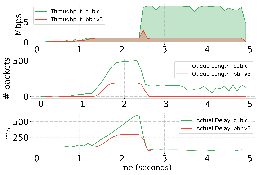
\includegraphics[width=78mm,height=52mm,keepaspectratio]{bbr-convergence.pdf}
\end{textblock*}
\begin{textblock*}{57mm}(95mm,26mm)
\raggedright\color[HTML]{142D45}\fontsize{10.7}{13.161}\selectfont \begin{itemize}\setlength{\itemsep}{2.6mm}\setlength{\parskip}{0pt}
\item Short run: BBR v3 stays low while CUBIC ramps up
\item Longer run: BBR v3 eventually increases throughput
\item Changing fq\_codel to fq did not remove slow convergence
\end{itemize}
\end{textblock*}
\end{frame}
\note{Why did this kernel TCP receive bug surface specifically when testing BBR? The authors attribute the triggering sequence to BBR's pacing behavior, which helped produce this particular packet-arrival order in their experiment. This also underscores the value of emulating real kernel code rather than testing simplified simulator models.\par \par When the authors re-tested on a newer Linux kernel (6.13.7+) from Google's BBR team, the earlier ACK bug did not appear in their tests. Even so, AdvNet found another scenario (Figure 6) where CUBIC quickly ramps up throughput while BBR v3 stays low during a short 5-second run. Extending the run showed that BBR v3 eventually ramps up—indicating a \textbf{slow convergence} issue rather than a permanent stall—and switching Mahimahi's queue discipline from `fq\_codel` to Google's recommended `fq` did not eliminate this behavior.
\par\smallskip Source: AdvNet paper §4.4.1, Fig.6}


% Slide 27: Fairness between competing flows
% AdvNet paper §3.5, §4.4.2
\begin{frame}[plain]
\begin{textblock*}{144mm}(8mm,6mm)
\raggedright\color[HTML]{142D45}\fontsize{22}{27.06}\selectfont \bfseries Fairness between competing flows
\end{textblock*}
\begin{textblock*}{144mm}(8mm,25mm)
\raggedright\color[HTML]{2869B3}\fontsize{12}{14.76}\selectfont \bfseries Fairness comparison
\end{textblock*}
\begin{textblock*}{144mm}(8mm,38mm)
\raggedright\color[HTML]{142D45}\fontsize{11}{13.53}\selectfont \setlength{\tabcolsep}{1.4mm}\renewcommand{\arraystretch}{1.35}
\begin{tabular}{@{}>{\raggedright\arraybackslash}p{70.600mm}>{\raggedright\arraybackslash}p{70.600mm}@{}}\toprule
\textbf{Reference score} & \textbf{Target score}\\
\midrule
Reference flow running alone & The same reference flow competing with a target\\
\bottomrule\end{tabular}
\end{textblock*}
\begin{textblock*}{51mm}(8mm,67mm)
\raggedright\color[HTML]{2869B3}\fontsize{24}{29.52}\selectfont \bfseries 40–80 s
\end{textblock*}
\begin{textblock*}{87mm}(65mm,66mm)
\raggedright\color[HTML]{142D45}\fontsize{11.5}{14.145}\selectfont Initially normal operation, then one packet at a time per ACK for the remaining 25–60 seconds.
\end{textblock*}
\end{frame}
\note{A second way to use UC1 is testing fairness between competing flows. Here, we define the reference score as the throughput of a reference protocol running alone on the link, and the target score as the throughput of that same reference flow when competing simultaneously against a target protocol. A high score means the competing flow severely starves the reference flow.\par \par While BBR is commonly perceived as dominating loss-based protocols like CUBIC, AdvNet discovered environments where CUBIC consumes nearly 100\% of the link bandwidth and starves BBR—and when their roles were reversed, AdvNet also found environments where BBR starves CUBIC.\par \par Digging into the logs, the authors found a striking pathology: the affected flow initially operates normally for 40 to 80 seconds, but then abruptly drops its sending rate to just a single packet at a time—waiting for an ACK before sending the next packet—for the remaining 25 to 60 seconds of the test. The authors reported this environment to the BBR development team, who confirmed the issue.
\par\smallskip Source: AdvNet paper §3.5, §4.4.2}


% Slide 28: Regression testing: BBR v1 and v3
% AdvNet paper §4.4.5; introduction
\begin{frame}[plain]
\begin{textblock*}{144mm}(8mm,6mm)
\raggedright\color[HTML]{142D45}\fontsize{22}{27.06}\selectfont \bfseries Regression testing: BBR v1 and v3
\end{textblock*}
\begin{textblock*}{144mm}(8mm,25mm)
\raggedright\color[HTML]{2869B3}\fontsize{12}{14.76}\selectfont \bfseries Dynamic trace, then 60 s fixed conditions; measure the final 10 s
\end{textblock*}
\begin{textblock*}{144mm}(8mm,43mm)
\raggedright\color[HTML]{142D45}\fontsize{12}{14.76}\selectfont \setlength{\tabcolsep}{1.4mm}\renewcommand{\arraystretch}{1.35}
\begin{tabular}{@{}>{\raggedright\arraybackslash}p{70.600mm}>{\raggedright\arraybackslash}p{70.600mm}@{}}\toprule
\textbf{Competing configuration} & \textbf{Reported throughput balance}\\
\midrule
CUBIC with BBR v1 & CUBIC / BBR v1 = 12\\
CUBIC with BBR v3 & BBR v3 / CUBIC = 11.6\\
\bottomrule\end{tabular}
\end{textblock*}
\begin{textblock*}{144mm}(8mm,80mm)
\raggedright\color[HTML]{526474}\fontsize{10.5}{12.915}\selectfont Single-flow tests also found BBR v1 throughput more than five times BBR v3.
\end{textblock*}
\end{frame}
\note{Moving to UC2, the authors used AdvNet for regression testing between BBR v1 and BBR v3, focusing on their fairness toward a competing CUBIC flow. In each candidate environment, they run two tests: first, CUBIC competing alongside BBR v1 (whose CUBIC throughput serves as the reference score), and second, CUBIC competing alongside BBR v3 (whose CUBIC throughput serves as the target score). To measure steady-state impact rather than transient jitter, AdvNet first varies bandwidth and latency, then holds the network conditions fixed for one minute, and measures throughput over the final ten seconds.\par \par In one adversarial environment discovered by AdvNet, when CUBIC competes with BBR v1, CUBIC achieves 12 times the throughput of BBR v1; yet when BBR v1 is replaced by BBR v3 under the exact same trace, the balance completely reverses, with BBR v3 achieving 11.6 times the throughput of CUBIC. In single-flow tests, AdvNet also found scenarios where BBR v1 achieves more than five times the throughput of BBR v3.\par \par Why do we see such dramatic reversals between versions? As the authors note, these outcomes are a direct consequence of the suboptimal BBR behaviors—such as rate collapse and slow convergence—uncovered in the earlier case studies. Even though BBR v3 was designed to improve fairness in typical settings, adversarial testing reveals specific dynamic conditions where version changes trigger severe regressions.
\par\smallskip Source: AdvNet paper §4.4.5; introduction}


% Slide 29: DChannel and early timeout estimates
% AdvNet paper §4.4.3
\begin{frame}[plain]
\begin{textblock*}{144mm}(8mm,6mm)
\raggedright\color[HTML]{142D45}\fontsize{22}{27.06}\selectfont \bfseries DChannel and early timeout estimates
\end{textblock*}
\begin{textblock*}{144mm}(8mm,25mm)
\raggedright\color[HTML]{142D45}\fontsize{11}{13.53}\selectfont \setlength{\tabcolsep}{1.4mm}\renewcommand{\arraystretch}{1.35}
\begin{tabular}{@{}>{\raggedright\arraybackslash}p{52.592mm}>{\raggedright\arraybackslash}p{34.600mm}>{\raggedright\arraybackslash}p{51.208mm}@{}}\toprule
\textbf{Path} & \textbf{One-way delay} & \textbf{Typical packets}\\
\midrule
High bandwidth (HBP) & 120 ms & Large data packets\\
Low latency (LLP) & 3 ms & Small control packets\\
\bottomrule\end{tabular}
\end{textblock*}
\begin{textblock*}{69mm}(8mm,63mm)
\raggedright\color[HTML]{2869B3}\fontsize{12}{14.76}\selectfont \bfseries Small early RTT estimate
\end{textblock*}
\begin{textblock*}{69mm}(8mm,76mm)
\raggedright\color[HTML]{142D45}\fontsize{11}{13.53}\selectfont The handshake uses the LLP.
\end{textblock*}
\begin{textblock*}{67mm}(85mm,63mm)
\raggedright\color[HTML]{C06821}\fontsize{12}{14.76}\selectfont \bfseries About 200 ms minimum RTO
\end{textblock*}
\begin{textblock*}{67mm}(85mm,76mm)
\raggedright\color[HTML]{142D45}\fontsize{11}{13.53}\selectfont HBP data can time out before its ACK.
\end{textblock*}
\end{frame}
\note{In UC3, the authors test a clear design objective for multipath transport: using two paths should never perform worse than using just one of those paths alone.\par \par They first evaluated \textbf{DChannel}, which combines a high-bandwidth path (HBP) and a low-latency path (LLP) in parallel while steering packets transparently below the transport layer. Here, the reference uses only the high-bandwidth path, the target uses DChannel over both paths, and the metric is flow completion time (FCT) for downloading a 20 MB file. Although prior work saw no issues when running loss-based CUBIC over DChannel, AdvNet found an environment—where the HBP has a 120 ms one-way delay and the LLP has only a 3 ms one-way delay—in which DChannel's throughput drops to one-third of using the HBP alone.\par \par The root cause lies in DChannel's packet-steering heuristic, which sends small control packets (such as TCP handshakes) over the fast LLP and large data packets over the slower HBP. Because the initial handshake completes over the 3 ms path, TCP estimates a tiny RTT and sets its retransmission timeout (RTO) to the Linux minimum of roughly 200 ms. When large data packets subsequently take the 120 ms one-way HBP, their round-trip and queuing delay exceeds the 200 ms RTO before ACKs can return—triggering spurious timeouts and rate reductions.
\par\smallskip Source: AdvNet paper §4.4.3}


% Slide 30: DChannel: two paths can finish later
% AdvNet paper §4.4.3, Fig.7
\begin{frame}[plain]
\begin{textblock*}{144mm}(8mm,6mm)
\raggedright\color[HTML]{142D45}\fontsize{22}{27.06}\selectfont \bfseries DChannel: two paths can finish later
\end{textblock*}
\begin{textblock*}{81mm}(8mm,27mm)
\raggedright\color[HTML]{142D45}\fontsize{11}{13.53}\selectfont 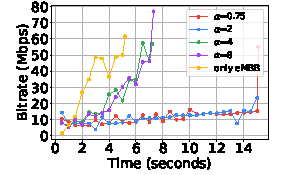
\includegraphics[width=81mm,height=49mm,keepaspectratio]{dchannel.pdf}
\end{textblock*}
\begin{textblock*}{54mm}(98mm,26mm)
\raggedright\color[HTML]{142D45}\fontsize{11}{13.53}\selectfont \begin{itemize}\setlength{\itemsep}{2.6mm}\setlength{\parskip}{0pt}
\item 20 MB file transfer
\item All tested alpha values finish later than the single HBP
\item Changing alpha softens the issue but does not remove it
\end{itemize}
\end{textblock*}
\end{frame}
\note{Figure 7 shows the download bitrate over time (where a curve ending earlier means the 20 MB file finished faster). DChannel steers a packet to the LLP only when its estimated reward exceeds $\alpha$ times its cost ($R > \alpha \times C$, with default $\alpha = 0.75$). As Fig. 7 shows, across all tested values of $\alpha$, DChannel takes much longer to finish than using the single high-bandwidth path (`only eMBB`). However, when the authors manually reduced the HBP's RTT below the 200 ms minimum RTO threshold, DChannel once again outperformed the single path—supporting the authors' diagnosis.
\par\smallskip Source: AdvNet paper §4.4.3, Fig.7}


% Slide 31: MPTCP: one path versus two
% AdvNet paper §4.4.4, Fig.8
\begin{frame}[plain]
\begin{textblock*}{144mm}(8mm,6mm)
\raggedright\color[HTML]{142D45}\fontsize{22}{27.06}\selectfont \bfseries MPTCP: one path versus two
\end{textblock*}
\begin{textblock*}{81mm}(8mm,30mm)
\raggedright\color[HTML]{142D45}\fontsize{11}{13.53}\selectfont 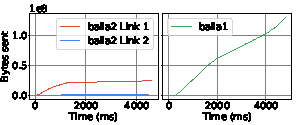
\includegraphics[width=81mm,height=39mm,keepaspectratio]{mptcp.pdf}
\end{textblock*}
\begin{textblock*}{54mm}(98mm,26mm)
\raggedright\color[HTML]{142D45}\fontsize{10.8}{13.284}\selectfont \begin{itemize}\setlength{\itemsep}{2.6mm}\setlength{\parskip}{0pt}
\item All four tested MPTCP algorithms have counterexamples
\item BALIA two-path throughput is 85.5\% lower in this example
\item A \textasciitilde{}40 ms ACK delay precedes the slowdown on both paths
\end{itemize}
\end{textblock*}
\end{frame}
\note{Finally, the authors tested the same "do no harm" objective on the Linux kernel implementation of \textbf{MPTCP} across all four of its congestion control algorithms: LIA, OLIA, BALIA, and wVegas. For every single one of them, AdvNet found environments where two paths yield lower throughput than one path.\par \par For BALIA (Figure 8), dual-path throughput (`balia2`) was 85.5\% lower than single-path throughput (`balia1`). Plotting cumulative bytes sent over time, `balia2` initially sends faster by using the high bandwidth of Link 1, but `balia1` overtakes it after about 0.5 seconds. Around 1.2 seconds, after the receiver delays an ACK by roughly 40 ms, `balia2` sharply reduces its sending rate on both links—even though Link 1 still has high available bandwidth.
\par\smallskip Source: AdvNet paper §4.4.4, Fig.8}


% Slide 32: What AdvNet contributes
% AdvNet paper §1–3
\begin{frame}[plain]
\begin{textblock*}{144mm}(8mm,6mm)
\raggedright\color[HTML]{142D45}\fontsize{22}{27.06}\selectfont \bfseries What AdvNet contributes
\end{textblock*}
\begin{textblock*}{144mm}(8mm,28mm)
\raggedright\color[HTML]{142D45}\fontsize{13}{15.99}\selectfont \begin{itemize}\setlength{\itemsep}{2.6mm}\setlength{\parskip}{0pt}
\item A shared search pipeline supports several developer tasks
\item Compact environments and noise handling contribute to its effectiveness
\item Representation, evaluation, and reference design deserve attention
\end{itemize}
\end{textblock*}
\end{frame}
\note{To wrap up, AdvNet turns worst-case protocol testing into an automated black-box search over real code in emulation. By pairing a compact interval representation and Post-Learning Selection with customizable reference comparisons, a single search pipeline can uncover Linux kernel bugs, catch version regressions, and validate multipath design goals. From an ML-for-systems perspective, the fact that GA, Bayesian optimization, and epsilon-greedy search achieve very similar scores in Fig. 3b highlights an important lesson: a compact environment representation and careful noise handling contribute to the framework's effectiveness, while optimizer complexity alone does not determine its performance. These experiments do not establish a universal ranking of their importance.
\par\smallskip Source: AdvNet paper §1–3}


% Slide 33: Scope and open questions
% AdvNet paper §5
\begin{frame}[plain]
\begin{textblock*}{144mm}(8mm,6mm)
\raggedright\color[HTML]{142D45}\fontsize{22}{27.06}\selectfont \bfseries Scope and open questions
\end{textblock*}
\begin{textblock*}{68mm}(8mm,25mm)
\raggedright\color[HTML]{2869B3}\fontsize{12}{14.76}\selectfont \bfseries Current boundaries
\end{textblock*}
\begin{textblock*}{68mm}(8mm,38mm)
\raggedright\color[HTML]{142D45}\fontsize{11.5}{14.145}\selectfont \begin{itemize}\setlength{\itemsep}{2.6mm}\setlength{\parskip}{0pt}
\item No estimate of deployment frequency
\item Manual root-cause diagnosis
\item Limited workload and loss dimensions
\end{itemize}
\end{textblock*}
\begin{textblock*}{67mm}(85mm,25mm)
\raggedright\color[HTML]{087F82}\fontsize{12}{14.76}\selectfont \bfseries Extensions
\end{textblock*}
\begin{textblock*}{67mm}(85mm,38mm)
\raggedright\color[HTML]{142D45}\fontsize{11.5}{14.145}\selectfont \begin{itemize}\setlength{\itemsep}{2.6mm}\setlength{\parskip}{0pt}
\item Richer environments and workloads
\item Characterize problematic environment regions
\item An ABR prototype already exists
\end{itemize}
\end{textblock*}
\end{frame}
\note{At the same time, AdvNet has clear boundaries. Its current model mainly varies link bandwidth, delay, duration, and buffer size, with continuous sending or a fixed transfer size. Packet loss arises implicitly from buffer limits; random loss and generated bursty cross-traffic are not explicit search dimensions. The framework neither estimates how often a counterexample occurs in real deployments nor automates root-cause diagnosis. Looking ahead, the framework could be extended to automatically characterize and summarize problematic regions of the environment space, with trace simplification as a possible additional extension, and applied to other dynamic systems such as adaptive bitrate video streaming, where the authors have already built a prototype.
\par\smallskip Source: AdvNet paper §5}


% Slide 34: Backup: formal methods and GANs
% AdvNet paper §6, Appendix D
\begin{frame}[plain]
\begin{textblock*}{144mm}(8mm,6mm)
\raggedright\color[HTML]{142D45}\fontsize{22}{27.06}\selectfont \bfseries Backup: formal methods and GANs
\end{textblock*}
\begin{textblock*}{68mm}(8mm,25mm)
\raggedright\color[HTML]{2869B3}\fontsize{12}{14.76}\selectfont \bfseries Formal methods
\end{textblock*}
\begin{textblock*}{68mm}(8mm,38mm)
\raggedright\color[HTML]{142D45}\fontsize{11.5}{14.145}\selectfont \begin{itemize}\setlength{\itemsep}{2.6mm}\setlength{\parskip}{0pt}
\item Specify properties and models
\item Can provide guarantees within those assumptions
\item Scaling to real kernel state is challenging
\end{itemize}
\end{textblock*}
\begin{textblock*}{67mm}(85mm,25mm)
\raggedright\color[HTML]{087F82}\fontsize{12}{14.76}\selectfont \bfseries GANs
\end{textblock*}
\begin{textblock*}{67mm}(85mm,38mm)
\raggedright\color[HTML]{142D45}\fontsize{11.5}{14.145}\selectfont \begin{itemize}\setlength{\itemsep}{2.6mm}\setlength{\parskip}{0pt}
\item Usually learn a data distribution
\item AdvNet has no challenging-trace dataset to imitate
\item Execution feedback drives a search for weaknesses
\end{itemize}
\end{textblock*}
\end{frame}
\note{\textbf{Formal verification} checks whether a system satisfies specified properties, using techniques such as model checking and symbolic analysis. These techniques typically require precise models or specifications and can struggle to scale to complex kernel implementations and large spaces of time-varying network conditions. AdvNet instead uses execution feedback to search for performance weaknesses in real implementations.\par \par \textbf{Generative Adversarial Networks (GANs)} typically learn to generate data resembling an existing dataset. For AdvNet, the challenge is that we do not already have a dataset of challenging network environments to imitate. The search instead creates these environments using the observed performance gap as feedback.
\par\smallskip Source: AdvNet paper §6, Appendix D}


% Slide 35: Backup: alternatives to MRE
% AdvNet paper §3.3, Appendix B
\begin{frame}[plain]
\begin{textblock*}{144mm}(8mm,6mm)
\raggedright\color[HTML]{142D45}\fontsize{22}{27.06}\selectfont \bfseries Backup: alternatives to MRE
\end{textblock*}
\begin{textblock*}{144mm}(8mm,27mm)
\raggedright\color[HTML]{142D45}\fontsize{12}{14.76}\selectfont \setlength{\tabcolsep}{1.4mm}\renewcommand{\arraystretch}{1.35}
\begin{tabular}{@{}>{\raggedright\arraybackslash}p{35.300mm}>{\raggedright\arraybackslash}p{105.900mm}@{}}\toprule
\textbf{Method} & \textbf{Budget allocation}\\
\midrule
RoundRobin & Equal allocation across candidates\\
OCBA & More measurements for uncertain or close contenders\\
MRE & Repeated elimination, then continued evaluation of survivors\\
\bottomrule\end{tabular}
\end{textblock*}
\end{frame}
\note{\textbf{RoundRobin} divides the evaluation budget equally among the candidate environments, then selects the one with the highest observed mean score.\par \par \textbf{Optimal Computing Budget Allocation (OCBA)} distributes evaluations adaptively to increase the probability of selecting the candidate with the highest true mean. It prioritizes candidates with greater uncertainty or scores close to the current best. Compared with RoundRobin, it focuses measurements where they can most help distinguish the leading candidates. Figure 11 compares these methods with MRE.
\par\smallskip Source: AdvNet paper §3.3, Appendix B}


% Slide 36: Backup: GA operator equations
% AdvNet paper §3.2.2
\begin{frame}[plain]
\begin{textblock*}{144mm}(8mm,6mm)
\raggedright\color[HTML]{142D45}\fontsize{22}{27.06}\selectfont \bfseries Backup: GA operator equations
\end{textblock*}
\begin{textblock*}{144mm}(8mm,25mm)
\raggedright\color[HTML]{142D45}\fontsize{14}{17.22}\selectfont \(\displaystyle c_i=\begin{cases}b_i,&k_1<i\leq k_2,\\a_i,&\text{otherwise}\end{cases}\)
\end{textblock*}
\begin{textblock*}{144mm}(8mm,51mm)
\raggedright\color[HTML]{142D45}\fontsize{13}{15.99}\selectfont \(\displaystyle m_i=\begin{cases}U_i,&\text{with probability }p,\\c_i,&\text{otherwise}\end{cases}\quad U_i\sim\operatorname{Unif}\{l_i,\ldots,u_i\}\)
\end{textblock*}
\begin{textblock*}{144mm}(8mm,78mm)
\raggedright\color[HTML]{526474}\fontsize{10}{12.3}\selectfont a, b: parents; c: child; m: mutated child; k\(_1\), k\(_2\): cut positions; lᵢ, uᵢ: bounds
\end{textblock*}
\end{frame}
\note{Here, $a$ and $b$ are the parent parameter vectors, and $i$ is a gene index. The cut points determine which coordinates the child takes from each parent. Mutation replaces each selected coordinate with a uniform integer sample from that coordinate's bounds.
\par\smallskip Source: AdvNet paper §3.2.2}


% Slide 37: Backup: the selection simulation
% AdvNet paper Appendix B, Fig.11
\begin{frame}[plain]
\begin{textblock*}{144mm}(8mm,6mm)
\raggedright\color[HTML]{142D45}\fontsize{22}{27.06}\selectfont \bfseries Backup: the selection simulation
\end{textblock*}
\begin{textblock*}{82mm}(8mm,27mm)
\raggedright\color[HTML]{142D45}\fontsize{11}{13.53}\selectfont 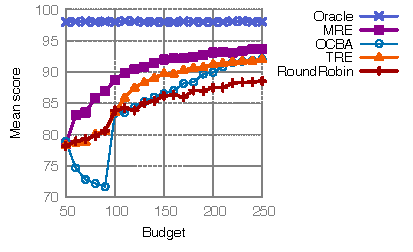
\includegraphics[width=82mm,height=50mm,keepaspectratio]{mre-simulation.pdf}
\end{textblock*}
\begin{textblock*}{53mm}(99mm,27mm)
\raggedright\color[HTML]{142D45}\fontsize{10.8}{13.284}\selectfont \begin{itemize}\setlength{\itemsep}{2.6mm}\setlength{\parskip}{0pt}
\item 50 Gaussian alternatives with means sampled from 0–100
\item The vertical axis is the true mean of the selected alternative
\item MRE leads among the tested methods under this statistical model
\end{itemize}
\end{textblock*}
\end{frame}
\note{This experiment (Appendix B, Fig. 11) uses fifty Gaussian alternatives, with their true means sampled uniformly between zero and one hundred. The vertical axis is the true mean of the alternative selected by each method, averaged over two thousand trials. The oracle knows those true means. MRE performs best among the tested selection methods under this model, whereas OCBA struggles at small budgets (< 100 samples) because there are not enough samples per candidate to estimate variance reliably. Note that these values use a different scale from the normalized protocol-gap score.
\par\smallskip Source: AdvNet paper Appendix B, Fig.11}


% Slide 38: Backup: parallel execution costs
% AdvNet paper Appendix A, Fig.9
\begin{frame}[plain]
\begin{textblock*}{144mm}(8mm,6mm)
\raggedright\color[HTML]{142D45}\fontsize{22}{27.06}\selectfont \bfseries Backup: parallel execution costs
\end{textblock*}
\begin{textblock*}{85mm}(8mm,24mm)
\raggedright\color[HTML]{142D45}\fontsize{11}{13.53}\selectfont 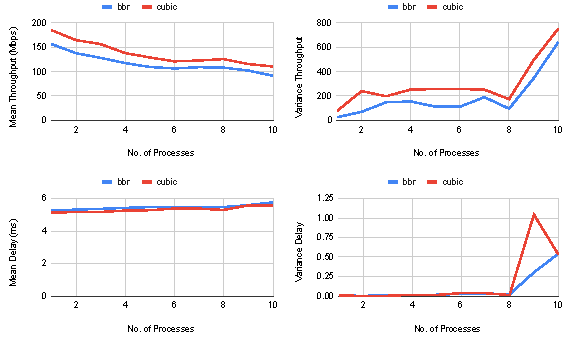
\includegraphics[width=85mm,height=51mm,keepaspectratio]{parallel-interference.pdf}
\end{textblock*}
\begin{textblock*}{51mm}(101mm,26mm)
\raggedright\color[HTML]{142D45}\fontsize{11}{13.53}\selectfont \begin{itemize}\setlength{\itemsep}{2.6mm}\setlength{\parskip}{0pt}
\item Three dedicated cores per execution
\item Throughput changes with parallelism
\item Variance rises at nine and ten executions
\end{itemize}
\end{textblock*}
\end{frame}
\note{To evaluate each candidate environment multiple times without increasing wall-clock time, AdvNet runs multiple Mahimahi instances in parallel, pinning 3 dedicated CPU cores per instance (one each for the emulator, `iperf` client, and `iperf` server).\par \par In Appendix A (Fig. 9), testing fixed network parameters (1 Gbps bandwidth, 5 ms one-way delay) on a 30-core server showed that mean throughput gradually drops as parallelism increases due to hardware contention, and variance spikes sharply at 9 and 10 concurrent runs (where $9 \times 3 = 27$ dedicated cores approaches the machine's 30-core count; this arithmetic alone does not establish CPU oversubscription). The authors therefore capped parallelism at 8.
\par\smallskip Source: AdvNet paper Appendix A, Fig.9}


% Slide 39: Backup: choosing the parallelism level
% AdvNet paper Appendix A, Fig.10
\begin{frame}[plain]
\begin{textblock*}{144mm}(8mm,6mm)
\raggedright\color[HTML]{142D45}\fontsize{22}{27.06}\selectfont \bfseries Backup: choosing the parallelism level
\end{textblock*}
\begin{textblock*}{76mm}(8mm,27mm)
\raggedright\color[HTML]{142D45}\fontsize{11}{13.53}\selectfont 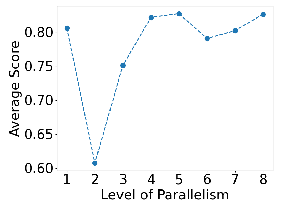
\includegraphics[width=76mm,height=52mm,keepaspectratio]{parallel-score.pdf}
\end{textblock*}
\begin{textblock*}{58mm}(94mm,27mm)
\raggedright\color[HTML]{142D45}\fontsize{11.5}{14.145}\selectfont \begin{itemize}\setlength{\itemsep}{2.6mm}\setlength{\parskip}{0pt}
\item More repetitions help with noise but add interference
\item Five-way evaluation gives the best score in this setup
\item The improvement over one evaluation is small
\end{itemize}
\end{textblock*}
\end{frame}
\note{In Fig. 10 (250 GA iterations), moving from 1 to 2 parallel runs initially lowers the final score because emulator contention distorts throughput during search (while the final output is always evaluated using a single isolated instance). Increasing parallelism further provides more samples to combat noise, peaking at 5-way parallelism—though the gain over a single evaluation per environment is marginal, so 1-way evaluation remains a practical low-CPU alternative.
\par\smallskip Source: AdvNet paper Appendix A, Fig.10}

\end{document}
